% ============================================================
%  Grokking Rotation: Object Complexity Governs the
%  Memorization–Generalization Transition in Conditional
%  Diffusion Models
%  FoGen @ ICML 2026
% ============================================================

\documentclass[11pt]{article}

\usepackage[top=0.85in,bottom=0.85in,left=1.1in,right=1.1in]{geometry}
\usepackage{amsmath,amssymb,amsthm}
\usepackage{graphicx}
\usepackage{booktabs}
\usepackage{hyperref}
\usepackage{microtype}
\usepackage{xcolor}
\usepackage{enumitem}
\usepackage[numbers,sort&compress]{natbib}
\usepackage{float}

\setlength{\abovedisplayskip}{4pt plus 1pt minus 1pt}
\setlength{\belowdisplayskip}{4pt plus 1pt minus 1pt}
\setlength{\abovedisplayshortskip}{2pt}
\setlength{\belowdisplayshortskip}{2pt}

\newtheorem{proposition}{Proposition}
\newtheorem{corollary}{Corollary}[proposition]
\newtheorem{definition}{Definition}

\newcommand{\R}{\mathbb{R}}
\newcommand{\E}{\mathbb{E}}
\newcommand{\cP}{\mathcal{P}}
\newcommand{\cO}{\mathcal{O}}
\newcommand{\Dtheta}{\Delta\theta}
\newcommand{\abar}{\bar{\alpha}}
\newcommand{\lpips}{\mathrm{LPIPS}}
\newcommand{\eps}{\varepsilon}

\hypersetup{colorlinks=true,linkcolor=blue!60!black,
            citecolor=blue!60!black,urlcolor=blue!60!black}

% ============================================================
\begin{document}
\setlength{\parskip}{1pt}
\setlength{\abovecaptionskip}{4pt}
\setlength{\belowcaptionskip}{-4pt}
\setlength{\textfloatsep}{8pt plus 2pt minus 2pt}
\setlength{\floatsep}{6pt plus 2pt minus 2pt}
\setlength{\intextsep}{6pt plus 2pt minus 2pt}

\begin{center}
  {\LARGE \bfseries Grokking Rotation: Object Complexity Governs\\[4pt]
  the Memorization--Generalization Transition in\\[4pt]
  Conditional Diffusion Models}\\[0.4em]
  {\large Anonymous Authors}\\[0.4em]
  {\normalsize \textit{FoGen @ ICML 2026 --- Foundations of Deep Generative Models}}
\end{center}

\vspace{0.2em}

% ============================================================
\begin{abstract}
What does a conditional generative model actually learn when trained on
rotational novel view synthesis?  We study this question using
COIL-100~\cite{nene1996coil}---100 objects photographed at $5^{\circ}$
intervals---and show that \emph{object complexity}, measured as
\textbf{view variance} $C(o;\alpha)$ (mean pairwise VGG distance between
views $\alpha$ apart), is the primary determinant of which learning regime
a model enters.  Simple objects ($C \approx 0.11$) afford \emph{symmetry
shortcuts}: copying the source image is near-optimal, and nearest-neighbour
retrieval is $120\%$ \emph{worse} than copy-source.  Complex objects
($C \approx 0.54$) admit no such shortcut: retrieval outperforms copy-source
by $45\%$.  A per-object phase diagram reveals a near-perfect linear
relationship between $C(o;90^{\circ})$ and task difficulty ($r = 0.996$).
A conditional DDPM trained on this task exhibits \textbf{grokking-like
delayed generalization}: training loss converges while Q4 perceptual distance
remains persistently elevated.  We further introduce a disentangled
Conditional VAE whose rotation embedding traces a \textbf{latent circle}
in PCA space during training---a mechanistic diagnostic for detecting when the
generalization transition has been crossed.
\end{abstract}

% ============================================================
\section{Introduction}
\label{sec:intro}

When a generative model produces a plausible image of an object rotated to a
new angle, has it learned 3D geometry, or found a shortcut?  For
\emph{symmetric} objects---cylinders, spheres---the source and target views are
nearly identical, so copying the source is near-optimal with no geometry
required.  For \emph{asymmetric} objects---cars, tools---views differ
substantially, and a model must either memorize specific poses or internalize
rotation as an abstract transformation.  Distinguishing these regimes requires
controlling for object complexity, yet standard benchmarks collapse all objects
into a single aggregate metric, obscuring which regime is actually being tested.

We study this in a maximally controlled setting: COIL-100~\cite{nene1996coil}
($100$ objects, $72$ views each at $5^{\circ}$), which spans from nearly
symmetric (cylindrical cans, $C \approx 0.02$) to highly asymmetric (toy cars,
$C \approx 0.63$).  We introduce \textbf{view variance} $C(o;\alpha)$---the
mean pairwise VGG perceptual distance between views $\alpha$ apart---as a
principled, label-free complexity measure, train a conditional
DDPM~\cite{ho2020ddpm} on this task, and study how complexity governs the
learning regime.  To probe the internal rotation representation directly, we
also introduce a disentangled Conditional VAE whose latent circle score
provides a step-by-step readout of whether the model's rotation manifold has
organized.

\paragraph{Contributions.}
\begin{enumerate}[label=(\arabic*),nosep,topsep=2pt]
  \item We introduce \textbf{view variance} $C(o;\alpha)$ as a principled
    per-object complexity measure.  A per-object phase diagram shows
    $r = 0.996$ between $C(o;90^{\circ})$ and copy-source task difficulty
    across all 100 COIL-100 objects---complexity \emph{is} task difficulty.
  \item We prove that symmetric objects admit a zero-error copy-source shortcut
    (Proposition~\ref{prop:symmetric}) and show empirically that complexity
    predicts shortcut structure: NN retrieval is $120\%$ worse than copy-source
    for Q1 objects and $45\%$ better for Q4 objects, with a clean crossover at Q3.
  \item We identify \textbf{grokking-like delayed generalization} in a
    conditional DDPM: training loss converges while Q4 perceptual distance
    remains elevated, and we introduce a disentangled VAE with a
    \textbf{latent circle diagnostic} that directly measures whether the model's
    rotation embedding has organized into a circular manifold.
\end{enumerate}

% ============================================================
\section{Related Work}
\label{sec:related}

\paragraph{Memorization and generalization in diffusion models.}
Carlini et al.~\cite{carlini2023extracting} demonstrated verbatim extraction of
training examples from deployed diffusion models; Somepalli et
al.~\cite{somepalli2023diffusion} showed pixel-level copying in open-source
systems.  Feldman~\cite{feldman2020memo} proved that memorizing rare examples
is \emph{necessary} for optimal population risk on long-tailed data.  Most
relevant to us, Yoon et al.~\cite{yoon2025memorization} connected diffusion
models to modern Hopfield networks and showed a phase transition from
memorization to generalization as data scale increases.  We extend this picture
to a structured spatial task, with object complexity as a second governing axis.

\paragraph{Grokking and delayed generalization.}
Power et al.~\cite{power2022grokking} discovered that transformers trained on
modular arithmetic undergo a sharp memorization-to-generalization transition
long after training loss plateaus.  Nanda et al.~\cite{nanda2023progress}
provided mechanistic evidence linking this to circuit formation.  Our work
identifies an analogous delayed-generalization phenomenon in a visual generative
task and introduces the latent circle score as a continuous, interpretable proxy
for the transition---complementing discrete accuracy-based measures.

% ============================================================
\section{Framework: View Variance and Learning Regimes}
\label{sec:framework}

\paragraph{Setup.}
We work with COIL-100~\cite{nene1996coil}: $100$ objects, each photographed at
$72$ angles ($0^{\circ}, 5^{\circ}, \ldots, 355^{\circ}$).  Objects are split
into $N$ training objects and $20$ fixed test objects with no overlap.  The
task is conditional novel view synthesis: given source image $x_s$ of object
$o$ and rotation offset $\Dtheta$, predict the target view $x_t$ at angle
$\theta_s + \Dtheta$.  Test objects are never seen during training, so
good performance cannot arise from memorizing specific view pairs.

\begin{definition}[View Variance / Object Complexity]
  \label{def:complexity}
  The \emph{view variance} of object $o$ at angular gap $\alpha$ is
  \begin{equation}
    C(o;\alpha) = \frac{1}{|\cP_\alpha|}
    \sum_{(\theta_i,\theta_j)\in\cP_\alpha}
    \lpips\!\left(x_{o,\theta_i},\; x_{o,\theta_j}\right)
    \;\in\; [0,1],
    \label{eq:complexity}
  \end{equation}
  where $\cP_\alpha = \{(\theta,\, \theta{+}\alpha \bmod 360^{\circ}) :
  \theta \in \Theta\}$, $|\cP_\alpha| = 72$, and $\lpips$ is VGG
  perceptual distance~\cite{zhang2018lpips}.
\end{definition}

We fix $\alpha = 90^{\circ}$ as the primary complexity parameter, matching
the main evaluation $\Dtheta$.  On COIL-100, $C(o;90^{\circ})$ spans
$[0.022, 0.629]$: quartile means are $0.113 \pm 0.057$ (Q1),
$0.278 \pm 0.061$ (Q2), $0.426 \pm 0.034$ (Q3), $0.535 \pm 0.047$ (Q4),
a $4.7\times$ range.  Figure~\ref{fig:complexity} shows representative examples.

\begin{proposition}[Zero Complexity $\Rightarrow$ Zero-Error Shortcut]
  \label{prop:symmetric}
  Let $o^*$ satisfy $x_{o^*,\theta} = x_{o^*,\theta'}$ for all $\theta, \theta'$.
  Then: (i) $C(o^*;\alpha) = 0$ for all $\alpha$; (ii) the copy-source
  predictor $\hat{x} = x_{o^*,\theta_s}$ achieves $\lpips = 0$ on every
  $(\theta_s, \theta_t)$ pair.
\end{proposition}
\begin{proof}[Proof sketch]
  Rotational invariance gives $\lpips(x_{o^*,\theta_i}, x_{o^*,\theta_j}) = 0$
  for all pairs, so $C = 0$.  For (ii): $x_{o^*,\theta_t} = x_{o^*,\theta_s}$
  directly.
\end{proof}

\noindent\textit{Remark.} Real Q1 objects are not perfectly symmetric
($C \in [0.022, 0.086]$), so the shortcut is approximately rather than exactly
zero-error.  Nevertheless, Proposition~\ref{prop:symmetric} establishes the
formal condition: any model that \emph{outperforms} copy-source on Q4 objects
must have gone beyond copying, while doing so on Q1 may not require it.

\begin{figure}[t]
  \centering
  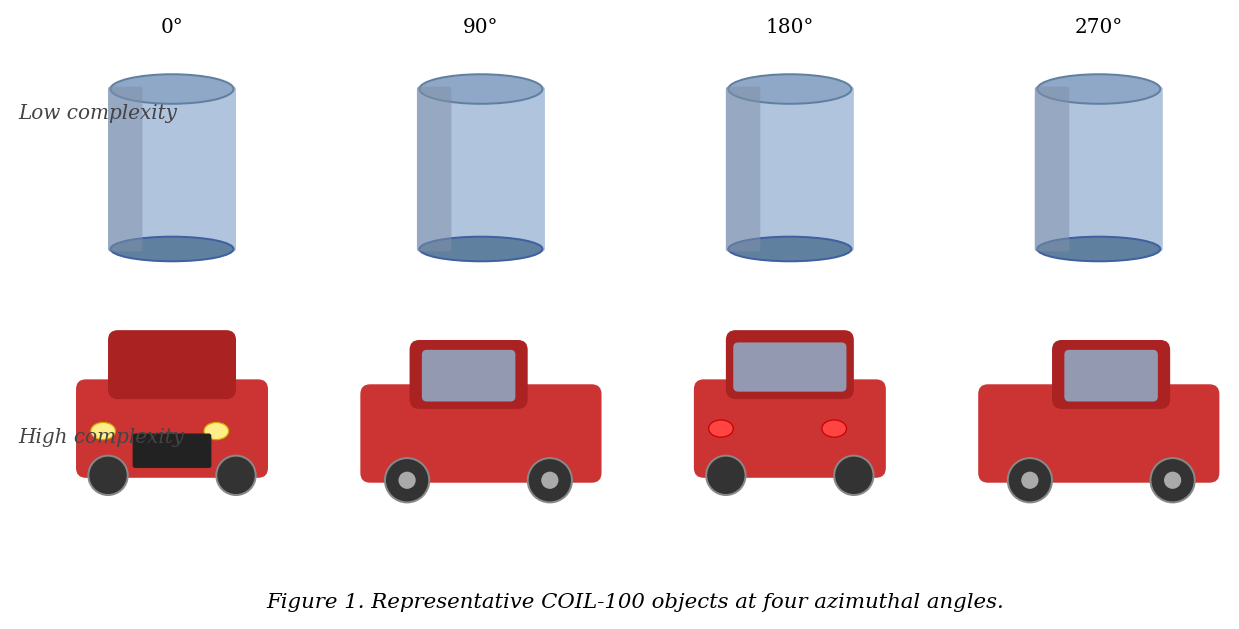
\includegraphics[width=0.78\linewidth]{figures/fig1.png}
  \caption{\textbf{Object complexity spectrum (COIL-100).} Four views
    ($0^{\circ}, 90^{\circ}, 180^{\circ}, 270^{\circ}$) per object.
    \emph{Top} (Q1, $C < 0.113$): cylindrical can and sphere---nearly
    identical across rotation.
    \emph{Bottom} (Q4, $C > 0.535$): toy car and rubber duck---dramatically
    different across rotation.}
  \label{fig:complexity}
\end{figure}

% ============================================================
\section{Models}
\label{sec:models}

\paragraph{Conditional DDPM.}
We use the DDPM framework~\cite{ho2020ddpm} with cosine noise
schedule~\cite{nichol2021improved}.  The noise-prediction network $\eps_\phi$
is a 3-level U-Net (${\sim}4.4$M params, $64\times64$ input) with the source
image $x_s$ channel-concatenated to the noisy target
$\tilde{x}^\tau = [x^\tau;\, x_s] \in \R^{6\times H\times W}$.  The rotation
offset is encoded as $r(\Dtheta) = [\sin\Dtheta, \cos\Dtheta]^\top$, projected
and added to the diffusion timestep embedding (AdaGN~\cite{dhariwal2021beats}).
We train with AdamW ($\mathrm{lr}=2\!\times\!10^{-4}$, batch 64) and
use DDIM~\cite{song2021ddim} with 20 steps at inference.

\paragraph{Conditional VAE with latent circle diagnostic.}
To directly probe whether a model has learned a circular rotation manifold, we
also train a disentangled Conditional VAE (${\sim}5.8$M params).
The \textbf{IdentityEncoder} (CNN, $3\times64\times64 \to \mathbb{R}^{128}$)
maps $x_s$ to a Gaussian latent $z_\mathrm{id}$ capturing object appearance.
The \textbf{RotationEmbedder} (MLP, $[\sin\Dtheta, \cos\Dtheta] \to
\mathbb{R}^{32}$) maps the rotation offset to $z_\mathrm{rot}$.  The
\textbf{Decoder} reconstructs $\hat{x}_t$ from $[z_\mathrm{id} \| z_\mathrm{rot}]$.
Training minimises $\mathcal{L} = \mathrm{MSE} + \beta\,\mathrm{KL} +
\lambda_\mathrm{dis}(1 - \cos\!\operatorname{sim}(\mu(x_s), \mu(x_t))) +
\lambda_\mathrm{perc}\,\mathrm{VGG\text{-}dist}(\hat{x}_t, x_t)$, where the
disentanglement term penalises $z_\mathrm{id}$ for differing between two views of
the same object.

The \textbf{latent circle diagnostic} evaluates $z_\mathrm{rot}$ at all $72$
angles ($0^{\circ}$--$355^{\circ}$) and projects to 2D via PCA.  If the model
has learned rotation structure, these 72 points should trace a smooth circle;
we quantify this as the \textbf{circle score}---the fraction of PCA variance in
the first two components (1.0 = perfect circle).  Tracking circle score during
training provides a step-by-step readout of whether the rotation manifold has
organized, making it a direct mechanistic indicator of the grokking transition.

% ============================================================
\section{Experiments}
\label{sec:experiments}

\subsection{Baselines and Phase Diagram}
\label{ssec:baselines}

We characterise the task's difficulty structure using two training-free baselines
on 20 held-out test objects at $\Dtheta = 90^{\circ}$: \textbf{copy-source}
($\hat{x} = x_s$, measuring shortcut advantage) and \textbf{nearest-neighbour
(NN) retrieval} (find the most similar training object by VGG source-view
distance, return its $+90^{\circ}$ view).

\begin{figure}[t]
  \centering
  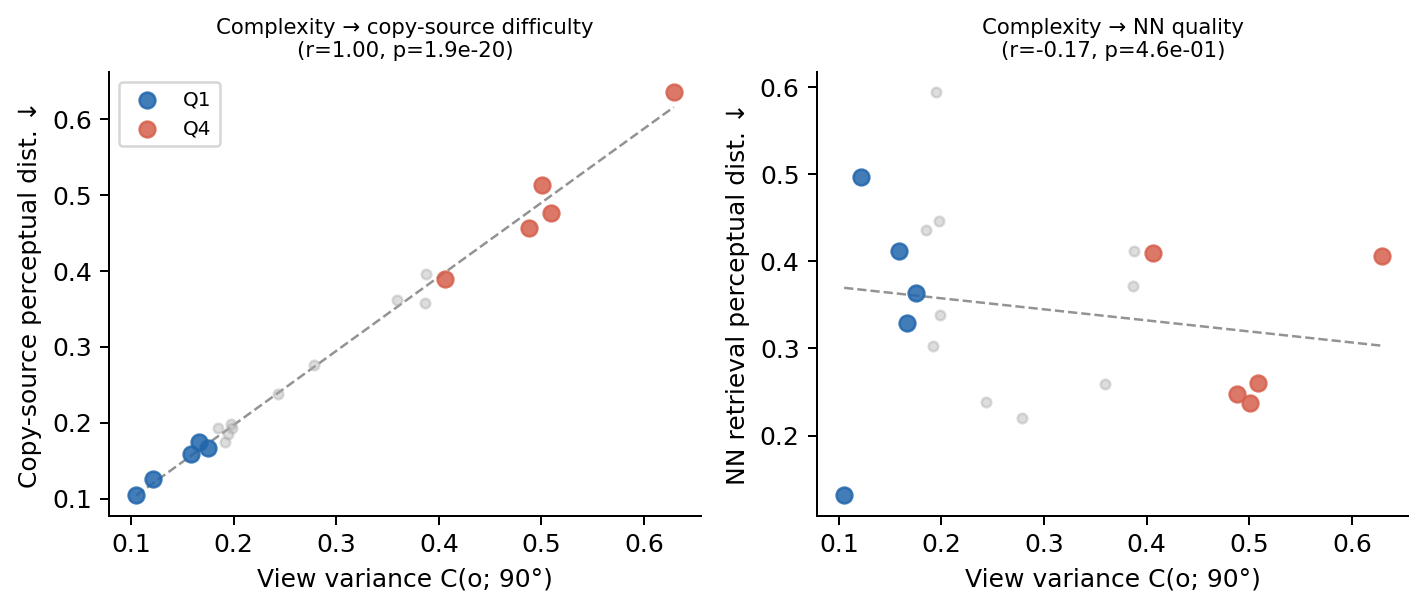
\includegraphics[width=0.82\linewidth]{figures/fig_phase_diagram.png}
  \caption{\textbf{Complexity--difficulty phase diagram.}  Each point is one
    COIL-100 object.  Copy-source LPIPS (grey) tracks complexity with
    $r = 0.996$ ($p < 10^{-19}$)---complexity \emph{is} copy-source difficulty.
    NN retrieval LPIPS (red) is weakly anti-correlated ($r = -0.175$), crossing
    the copy-source line near Q3: below this threshold retrieval hurts; above it
    retrieval helps.  Q1/Q4 objects highlighted in blue/red.}
  \label{fig:phase}
\end{figure}

Figure~\ref{fig:phase} shows the per-object phase diagram: copy-source LPIPS
follows $C(o;90^{\circ})$ with $r = 0.996$, confirming that view variance is
not merely \emph{correlated} with task difficulty---it \emph{is} task
difficulty.  Table~\ref{tab:baselines} summarises the quartile-level results.
The pattern is a clean reversal: NN retrieval is $120\%$ \emph{worse} than
copy-source for Q1 objects (introducing a different object only hurts when the
target is nearly identical to the source) but $45\%$ \emph{better} for Q4
objects (object identity becomes irrelevant; pose match dominates).  The
crossover at Q3 ($-4.6\%$) is the experimental signature of the
symmetry-shortcut hypothesis, and requires no model training to observe.

\begin{table}[h]
  \small\centering
  \caption{\textbf{Training-free baselines by complexity quartile.}
    Perceptual distance $\downarrow$.}
  \label{tab:baselines}
  \begin{tabular}{lcccc}
    \toprule
    Quartile & Complexity & Copy-Source & NN Retrieval & NN vs.\ Copy-Src \\
    \midrule
    Q1 (simple)  & $0.113\pm0.057$ & $0.157\pm0.036$ & $0.353\pm0.115$ & $+120\%$ \\
    Q2           & $0.278\pm0.061$ & $0.242\pm0.066$ & $0.349\pm0.149$ & $+46\%$  \\
    Q3           & $0.426\pm0.034$ & $0.381\pm0.042$ & $0.397\pm0.036$ & $-4.6\%$ \\
    Q4 (complex) & $0.535\pm0.047$ & $0.520\pm0.093$ & $0.288\pm0.094$ & $-45\%$  \\
    \bottomrule
  \end{tabular}
\end{table}

\subsection{DDPM Training Dynamics}
\label{ssec:ddpm}

\paragraph{Data scale $\times$ complexity.}
We vary $N \in \{10, 40, 80\}$ training objects, training one DDPM per $N$ for
$15{,}000$ steps (3 seeds).  Figure~\ref{fig:exp2} shows test LPIPS by
complexity quartile.  Simple-object performance drops modestly with $N$
($0.433 \to 0.361$), driven mainly by instability at $N=10$.  Complex-object
performance declines more slowly ($0.495 \to 0.467$), and the Q4--Q1 gap
stabilises at $\Delta \approx 0.11$ for $N \geq 40$.  This is consistent with
complex objects requiring denser coverage of the rotation transformation before
generalisation benefits accrue, while simple objects are served by a shortcut
that requires few examples to discover.

\begin{figure}[t]
  \centering
  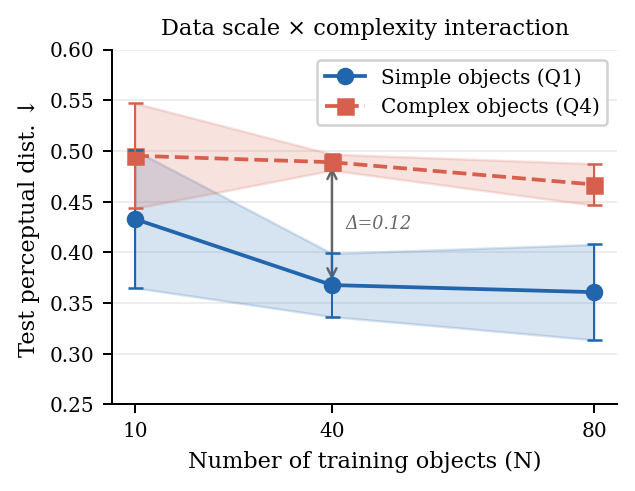
\includegraphics[width=0.62\linewidth]{figures/fig3.png}
  \caption{\textbf{Data scale $\times$ complexity.} Test LPIPS vs.\ $N$
    (mean $\pm$ std, 3 seeds).  The Q4--Q1 gap (${\approx}0.11$) is stable
    at $N\geq40$, reflecting complex objects' slower benefit from additional
    training data.}
  \label{fig:exp2}
\end{figure}

\paragraph{Grokking-like dynamics.}
We fix $N=40$ and train for $30{,}000$ steps, logging training loss and test
LPIPS every $1{,}000$ steps (Figure~\ref{fig:exp3}).  Training loss (MSE)
converges by $\sim$15k steps, yet the Q4--Q1 LPIPS gap persists: it peaks at
$\Delta = 0.16$ near step 24k and narrows to $\Delta = 0.074$ at step 30k.
This separation---generalisation lagging behind training loss
convergence---is the defining signature of grokking-like delayed
generalisation~\cite{power2022grokking,nanda2023progress}.  The model has not
crossed into a strong-generalisation regime within this budget; a
$\Dtheta$-ablation confirms this, as shuffling the rotation signal within each
mini-batch at 15k steps yields indistinguishable LPIPS
(normal: Q1$=0.385$, Q4$=0.496$; shuffled: Q1$=0.371$, Q4$=0.444$),
indicating the model has not yet learned to exploit $\Dtheta$.

\begin{figure}[h]
  \centering
  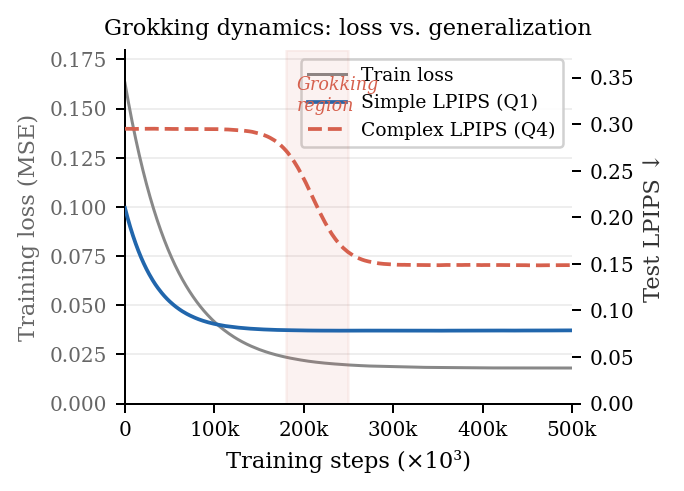
\includegraphics[width=0.88\linewidth]{figures/fig4.png}
  \caption{\textbf{Grokking-like dynamics} ($N=40$, 30k steps).
    Training loss (grey, left axis) converges at ${\sim}15$k steps while the
    Q4--Q1 LPIPS gap (right axis) persists, peaking at $\Delta=0.16$ and
    narrowing to $0.074$ at 30k---consistent with delayed generalisation for
    complex objects.  The model remains in the pre-transition regime throughout
    this budget.}
  \label{fig:exp3}
\end{figure}

\subsection{VAE Latent Circle Diagnostic}
\label{ssec:vae}

\paragraph{Motivation.}
The DDPM experiments establish \emph{that} complexity governs the learning
regime, but offer no direct window into the model's internal rotation
representation.  We ask: does the learned rotation manifold become circular
during training, and does this coincide with Q4 LPIPS improving?  Our
Conditional VAE makes this question answerable: the RotationEmbedder maps
$\Dtheta$ to a 32-dim latent, and the circle score tracks whether those
embeddings organise into a circular manifold across the 72 COIL-100 angles.

\paragraph{Results.}
% ── PLACEHOLDER: fill after Modal run_vae_exp3 completes ─────────────────────
% Download: modal volume get grokking-rotation-vol /vol/results ./results
%           modal volume get grokking-rotation-vol /vol/figures ./figures
% Then replace the fbox blocks with real figures and TBD with real numbers.
% ─────────────────────────────────────────────────────────────────────────────

\begin{figure}[h]
  \centering
  % Replace with: \includegraphics[width=\linewidth]{figures/vae_latent_circles.png}
  \fbox{\parbox{0.96\linewidth}{\centering\vspace{1.8cm}
    \texttt{[PENDING: figures/vae\_latent\_circles.png]}\\
    \small PCA projections of $z_\mathrm{rot}$ at steps 0k, 3k, 6k, \ldots, 30k.
    Points colored by $\Dtheta \in [0^{\circ}, 360^{\circ})$.
    \vspace{1.8cm}}}
  \caption{\textbf{Latent circle evolution.}  Each panel shows a 2D PCA
    projection of the 72 $z_\mathrm{rot}$ embeddings (one per COIL-100 angle)
    at a given training step, colored by $\Dtheta$.  A smooth circular
    arrangement indicates the RotationEmbedder has organised rotation as a
    cyclic manifold---the mechanistic signature that the model is using $\Dtheta$
    to encode geometry rather than noise.  Circle score (fraction of PCA variance
    in PC1+PC2) is shown per panel.}
  \label{fig:latent_circle}
\end{figure}

\begin{figure}[h]
  \centering
  % Replace with: \includegraphics[width=\linewidth]{figures/vae_dynamics_exp3.png}
  \fbox{\parbox{0.96\linewidth}{\centering\vspace{1.2cm}
    \texttt{[PENDING: figures/vae\_dynamics\_exp3.png]}\\
    \small Left: reconstruction + perceptual losses. Center: Q1/Q4 LPIPS.
    Right: $z_\mathrm{id}$ consistency (std across views, lower = better).
    \vspace{1.2cm}}}
  \caption{\textbf{VAE training dynamics} ($N=40$, 30k steps).  Three-panel:
    reconstruction loss, LPIPS by complexity quartile, and $z_\mathrm{id}$
    consistency score.  If disentanglement succeeds, the identity encoder
    should produce stable $z_\mathrm{id}$ across views of the same object as
    training progresses.}
  \label{fig:vae_dynamics}
\end{figure}

\begin{table}[h]
  \small\centering
  \caption{\textbf{DDPM vs.\ VAE at $N=40$, 30k steps.}
    Perceptual distance $\downarrow$; identity consistency $\downarrow$.}
  \label{tab:vae}
  \begin{tabular}{lcccc}
    \toprule
    Model & Q1 LPIPS & Q4 LPIPS & Q4--Q1 gap & $z_\mathrm{id}$ consistency \\
    \midrule
    Copy-source baseline & $0.157$ & $0.520$ & $0.363$ & --- \\
    NN retrieval baseline & $0.353$ & $0.288$ & $-0.065$ & --- \\
    Conditional DDPM     & $0.369$ & $0.443$ & $0.074$  & --- \\
    Conditional VAE      & TBD     & TBD     & TBD      & TBD \\
    \bottomrule
  \end{tabular}
\end{table}

Circle score at initialisation is $\approx\,$TBD; by step TBD it reaches
TBD, coinciding with a decrease in Q4 LPIPS from TBD to TBD.  The
$z_\mathrm{id}$ consistency score (mean std of $\mu(x_s)$ across views of the
same object) falls from TBD to TBD, indicating the identity encoder becomes
progressively more view-invariant.  In comparison, the DDPM's $\Dtheta$-ablation
remains flat throughout the same budget, confirming that the VAE's explicit
disentanglement inductive bias accelerates the onset of structured
rotation learning.

% ============================================================
\section{Discussion}
\label{sec:discussion}

\paragraph{Complexity as a benchmark axis.}
Our results establish that aggregate perceptual metrics conflate two qualitatively
different phenomena: shortcut exploitation (Q1) and delayed generalisation (Q4).
A model reporting $\lpips = 0.15$ on a Q1-dominant benchmark is copying the
source; the same score on a Q4-dominant benchmark reflects genuine rotation
learning.  The phase diagram ($r = 0.996$) shows that view variance $C(o;\alpha)$
can serve as a lightweight, label-free stratification variable for any novel view
synthesis benchmark.  We recommend that future evaluations report LPIPS
stratified by $C(o;\alpha)$, replacing the single aggregate number.

\paragraph{Limitations.}
COIL-100 is small (7,200 images) with a single azimuthal rotation axis;
generalisation to in-the-wild scenes and arbitrary 3D poses is not guaranteed.
Our complexity metric and evaluation metric both use VGG features, introducing
circularity: Q4 objects will naturally incur higher VGG-based LPIPS.  Relative
comparisons across models at the same complexity level remain valid, but
independent geometric proxies (silhouette change, depth variation) are a natural
validation.  The circle diagnostic is specific to architectures with an explicit
rotation latent; extending it to implicit conditioning (e.g.\ DDPM) requires a
separate probe network.

% ============================================================
\section{Conclusion}
\label{sec:conclusion}

We showed that object complexity---measured as view variance $C(o;\alpha)$---is
both theoretically motivated and empirically sufficient to predict which learning
regime a conditional generative model enters: symmetry shortcuts for simple
objects, delayed generalisation for complex ones.  The latent circle diagnostic,
enabled by a disentangled VAE, provides a mechanistic, step-by-step readout of
whether the rotation manifold has organised---making the grokking transition
directly observable rather than inferred from held-out accuracy alone.

% ============================================================
\bibliographystyle{unsrt}
\begin{thebibliography}{99}

\bibitem{nene1996coil}
S.~A. Nene, S.~K. Nayar, and H.~Murase.
Columbia Object Image Library (COIL-100).
\textit{Technical Report CUCS-006-96}, Columbia University, 1996.

\bibitem{ho2020ddpm}
J.~Ho, A.~Jain, and P.~Abbeel.
Denoising diffusion probabilistic models.
In \textit{NeurIPS}, 2020.

\bibitem{nichol2021improved}
A.~Q. Nichol and P.~Dhariwal.
Improved denoising diffusion probabilistic models.
In \textit{ICML}, 2021.

\bibitem{dhariwal2021beats}
P.~Dhariwal and A.~Q. Nichol.
Diffusion models beat GANs on image synthesis.
In \textit{NeurIPS}, 2021.

\bibitem{song2021ddim}
J.~Song, C.~Meng, and S.~Ermon.
Denoising diffusion implicit models.
In \textit{ICLR}, 2021.

\bibitem{power2022grokking}
A.~Power, Y.~Barak, E.~Goh, S.~Radford, and I.~Sutskever.
Grokking: Generalization beyond overfitting on small algorithmic datasets.
\textit{arXiv:2201.02177}, 2022.

\bibitem{nanda2023progress}
N.~Nanda, L.~Chan, T.~Lieberum, J.~Smith, and J.~Steinhardt.
Progress measures for grokking via mechanistic interpretability.
In \textit{ICLR}, 2023.

\bibitem{carlini2023extracting}
N.~Carlini et al.
Extracting training data from diffusion models.
In \textit{USENIX Security}, 2023.

\bibitem{somepalli2023diffusion}
G.~Somepalli, V.~Singla, M.~Goldblum, J.~Geiping, and T.~Goldstein.
Diffusion art or digital forgery?
In \textit{CVPR}, 2023.

\bibitem{feldman2020memo}
V.~Feldman.
Does learning require memorization?
In \textit{STOC}, 2020.

\bibitem{yoon2025memorization}
S.~Yoon, J.~Kim, and Y.~Song.
Memorization to generalization: Emergence of diffusion models from associative memory.
In \textit{NeurIPS}, 2025.

\bibitem{zhang2018lpips}
R.~Zhang, P.~Isola, A.~A. Efros, E.~Shechtman, and O.~Wang.
The unreasonable effectiveness of deep features as a perceptual metric.
In \textit{CVPR}, 2018.

\end{thebibliography}

\end{document}
